\chapter{Hintergrund}\label{ch:hintergrund}
%Begriffsklärung, Mathematische Grundlagen und grundlegende Algorithmen
%Wenn Sie mehrere bekannte Verfahren/Algorithmen in ihrer Arbeit verwenden und verketten, sollten sie die Verfahren hier zunächst erklären, so dass der Hauptteil später nicht permanent von Erklärungen einzelner Algorithmen unterbrochen wird. Auch mathematische Grundlagen können hier kurz zusammengefasst werden.
Im Folgenden werden grundlegende Begriffe, mathematische und probabilistische Verfahren sowie Daten- und Indexstrukturen dargestellt, die Eingang in diese Arbeit gefunden haben. Es wird erläutert, inwiefern sie für das soziale Netzwerk AMBIENCE relevant sind oder darin verwendet werden. 
\section{Bloom-Filter}\label{sec:bloom}
Ein Bloom-Filter ist eine probabilistische Datenstruktur zur Beschreibung von Mengen, die in der ursprünglichen From 1970 von Burton H. Bloom eingeführt wurde\footnote{Vgl. \cite{Bloom1970}.}. Er besteht aus einem Bit-Array der festen Länge \textit{m}, dessen Elemente zunächst alle auf 0 gesetzt sind. Das Einfügen von Informationsobjekten basiert auf der Berechnung einer festen Anzahl \textit{k} unabhängiger Hashfunktionen, die positive Werte kleiner als \textit{m} annehmen. Soll ein Objekt in den Filter eingefügt werden, werden seine Hashwerte berechnet und die die entsprechenden Bits im Filter gesetzt\footnote{Vgl. \cite{Broder2004}: 487.}. 

Die Hashwerte werden verwendet, um Anfragen auf dem Filter auszuführen. Ist ein Objekt im Filter enthalten, sind seine Bits gesetzt worden, d.h. man kann eine Anfrage nach seinen Hashwerten durchführen und so mit großer Wahrscheinlichkeit ermitteln, ob es in den Filter eingefügt wurde: Sind ein oder mehrere Bits des Anfrageobjekts nicht gesetzt, so ist das Element mit Sicherheit nicht vorhanden. Es gibt also keine falsch negativen Antworten. Allerdings kann es sein, dass ein Element nicht in den Filter eingefügt wurde, obwohl alle seine Bits gesetzt sind (falsch positive Antworten). Grund dafür ist die Kollisionseigenschaft von Hashfunktionen, die ein großes Universum von Elementen auf einen sehr viel kleineren Wertebereich, hier die Länge des Bloom-Filters, abbilden. Es kann somit zu Kollisionen zwischen unterschiedlichen Informationsobjekten bzw. ihren charakteristischen Hashwerten kommen. Die Falsch-Positiv-Rate eines Bloom-Filters ist abhängig von \textit{m}, \textit{k} und der Anzahl der eingefügten Elemente \textit{n} und lässt sich berechnen als\footnote{Vgl. ebd. für eine umfassende Darstellung.}
\[f = \left(1 - \left(1-\frac{1}{m}\right)^{kn}\right)^k.\]
Aus der Kollisionseigenschaft folgt auch, dass ein einmal eingefügtes Objekt nicht mehr aus einem Bloom-Filter gelöscht werden kann, weil das offensichtlich zu falsch negativen Ergebnissen für andere Objekte führen könnte. 
\begin{figure}[hpbt]
  \centering
  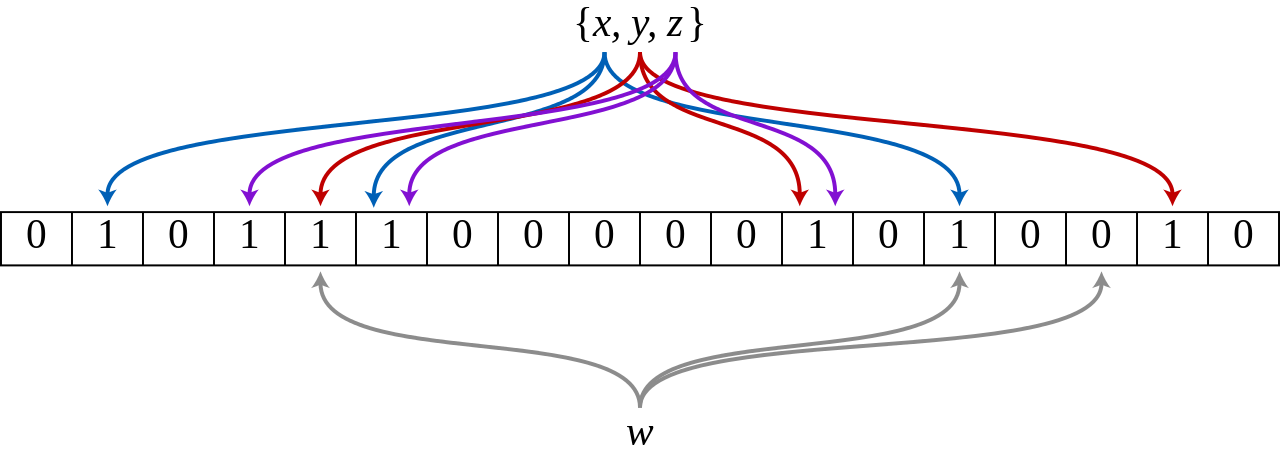
\includegraphics[width=0.8\textwidth]{pictures/1280px-Bloom_filter.png}\\
  \caption[Bloomfilter-Beispiel, Bildnachweis: \url{https://commons.wikimedia.org/wiki/File:Bloom_filter.svg}.]{Beispiel für einen Bloomfilter, in den die Objekte \textit{x}, \textit{y} und \textit{z} eingefügt wurden. Das Objekt \textit{w} ist nicht im Filter vorhanden.}\label{fig:pic0}
\end{figure}
\subsection{Distanzmaße und Teilmengenbeziehung}\label{sec:bloom-operationen}
Um die Ähnlichkeit zweier Mengen zu ermitteln, werden verschiedene Distanzmetriken oder Ähnlichkeitsmaße eingesetzt. Um Bloom-Filter miteinander zu vergleichen und insbesondere für die \textit{k}-nächste-Nachbarn-Suche muss ein geeignetes Ähnlichkeitsmaß zur Anwendung kommen. Bayardo et al. verwenden dazu die \textit{Kosinus-Ähnlichkeit}\footnote{Vgl. \cite{Bayardo2007}.}. Sakuma und Sato definieren die Ähnlichkeit von Bloom-Filtern über die Anzahl gleicher 1-Bits\footnote{Vgl. \cite{Sakuma2011}: 321.}. Ist diese für zwei Anfragefilter identisch, werden die Bit-Arrays negiert und die Anzahl gleicher 0-Bits verglichen. 

AMBIENCE verwendet eine Abschätzung der \textit{Jaccard-Distanz} zur Ermittlung der Ähnlichkeit von Bloom-Filtern. Die Jaccard-Distanz zwischen zwei Mengen \textit{A} und \textit{B} ist definiert als 
\[J_{\delta}(A,B) = 1 - J(A,B) = \frac{|A\cap B| - |A\cup B|}{|A\cup B|}, \]
wobei 
\[J(A,B) = \frac{|A\cap B|}{|A\cup B|}\] den \textit{Jaccard-Koeffizienten} bezeichnet. Die Jaccard-Distanz nimmt Werte im Bereich $\left[0,1\right]$ an. Identische Mengen haben eine Jaccard-Distanz von \textit{0}, Mengen ohne gemeinsame Elemente haben die Jaccard-Distanz \textit{1}. 
Für Bloom-Filter lässt sich die Jaccard-Distanz analog berechnen. Die Vereinigungsmenge zweier Bloom-Filter \textit{F} und \textit{G} lässt sich als bitweises logisches Oder, die Schnittmenge als bitweises logisches Und repräsentieren. Auch hier nimmt die Jaccard-Distanz offensichtlich Werte zwischen \textit{0} und \textit{1} an. Je ähnlicher die Filter sind, desto kleiner ist ihre Jaccard-Distanz. 
Die Jaccard-Distanz zwischen Bloom-Filtern ist, anders als die von Sakuma und Sato verwendete Distanz-Metrik, nicht transitiv in dem Sinne, dass zwei Filter, die beide eine geringe Jaccard-Distanz zu einem dritten Filter aufweisen, untereinander nicht ähnlich sein müssen. Man betrachte z.B. die Filter \textit{F1}, \textit{F2} und \textit{F3} mit folgenden Werten: 
\begin{figure}[hpbt]
  \centering
  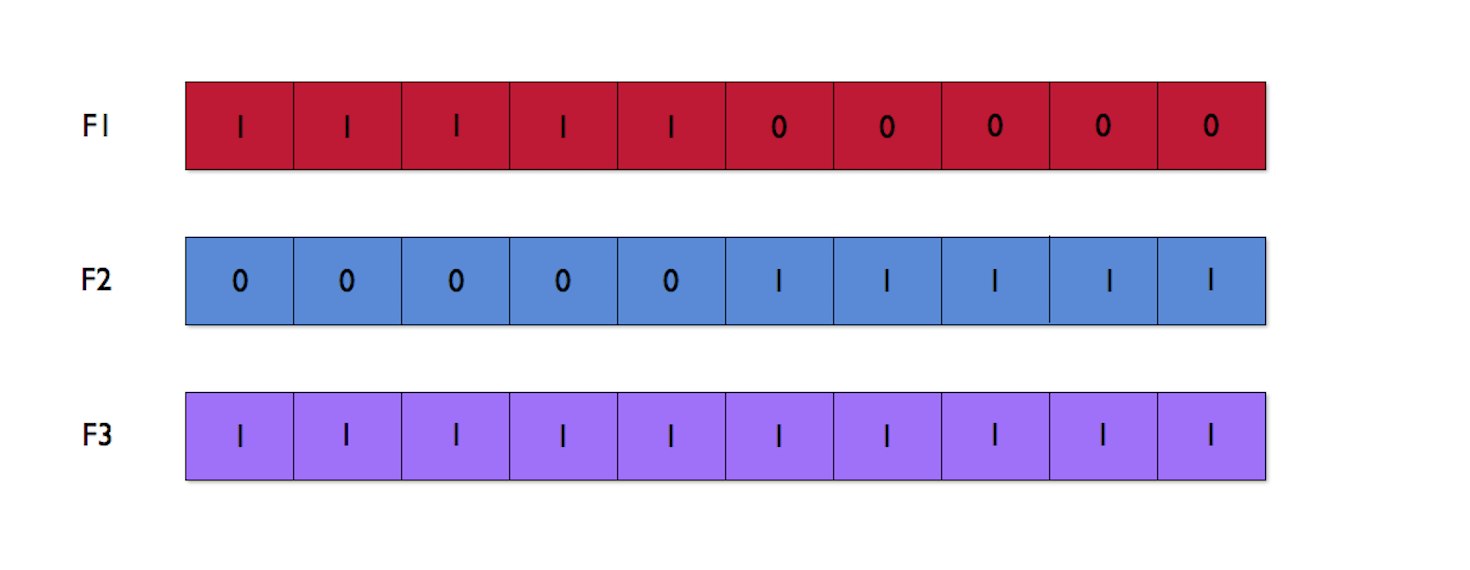
\includegraphics[width=1.0\textwidth]{pictures/filters.png}\\
  \caption[Jaccard-Distanzen zwischen Bloom-Filtern]{Jaccard-Distanzen zwischen Bloom-Filtern.}\label{fig:pic1}
\end{figure}
\newpage
\noindent
Die Jaccard-Distanzen zwischen \textit{F1}, \textit{F2} und \textit{F3} betragen somit: 
\[J_{\delta}(F1,F3) = 1 - J(F1,F3) = 1 - \frac{|F1\cap F3|}{|F1\cup F3|} = 1 - \frac{5}{10} = 0.5\]
\[J_{\delta}(F2,F3) = 1 - J(F2,F3) = 1 - \frac{|F2\cap F3|}{|F2\cup F3|} = 1 - \frac{5}{10} = 0.5\]
\[J_{\delta}(F1,F2) = 1 - J(F1,F2) = 1 - \frac{|F1\cap F2|}{|F1\cup F2|} = 1 - 0 = 1\]
Daran wird deutlich: Obwohl \textit{F1} und \textit{F2} jeweils die Hälfte der Elemente mit \textit{F3} gemeinsam haben, lässt sich daraus kein Wert für die Ähnlichkeit zwischen \textit{F1} und \textit{F2} ableiten. Sie sind sich im Gegenteil maximal unähnlich. 
\subsection{Hashfunktionen}\label{sec:hashfunktionen}
Die Frage, welche Hashfunktionen optimalerweise für einen Bloom-Filter verwendet werden sollten, ist nicht eindeutig zu beantworten\footnote{Vgl. \cite{Broder2004}: 487.}. Grundsätzlich muss zwischen kryptografischen Hashfunktionen wie MD5 und SHA und gewöhnlichen Hashfunktionen wie Murmur- oder Jenkins-Hashfunktionen unterschieden werden. Die Berechnung von kryptografischen Hashfunktionen dauert in der Regel länger, dafür haben sie bestimmte Eigenschaften wie eine hohe Kollisionsresistenz und Gleichverteilung der Ergebniswerte. 

Werden Bloom-Filter z.B. zum schnellen Nachschlagen in großen, verteilten Datenbanken eingesetzt, wird auf die kryptografischen Eigenschaften zu Gunsten des verminderten Rechenaufwandes verzichtet. Das NoSQL-Datenbanksystem Cassandra und das Hadoop-Framework für skalierte, verteilt arbeitende Software verwenden beispielsweise Bloom-Filter in Kombination mit Murmur- und Jenkins-Hashfunktionen. Darüber hinaus ist MD5 für Bloom-Filter weit verbreitet. Die Murmur-Hashfunktionen weisen gleichzeitig gute Verteilungseigenschaften auf und lassen sich vergleichsweise schnell berechnen, weswegen sie generell für den Einsatz in Bloom-Filtern empfohlen werden\footnote{Vgl. \url{http://spyced.blogspot.de/2009/01/all-you-ever-wanted-to-know-about.html}.}. AMBIENCE verwendet Murmur-Hashfunktionen zur Generierung der Bloom-Filter. Für die eigene Implementierung wurde der Murmur2-Hash verwendet\footnote{Vgl. \url{https://sites.google.com/site/murmurhash/MurmurHash2.cpp} für den Quellcode.}.  
\subsection{Varianten und Anwendungen}\label{sec:bloom-anwendungen}
Bloom-Filter erfreuen sich in verschiedenen Versionen großer Beliebtheit. Wichtige Varianten sind \textit{Attenuated Bloom Filter}\footnote{Vgl. \cite{Sakuma2011}: 316 und 318.}, \textit{Counting Bloom Filter}\footnote{Vgl. \cite{Fan2000}.} und \textit{Compressed Bloom Filter}\footnote{Vgl. \cite{Mitzenmacher2002}.}. Wegen der guten Kompressionseigenschaften und des geringen Speicherbedarfs kommen Bloom-Filter häufig in verteilten Anwendungen und Netzwerkdiensten zum Einsatz\footnote{Vgl. \cite{Broder2004} für eine ausführliche Darstellung.}. 

\noindent
Neben Hadoop und Cassandra werden Bloom-Filter in unzähligen, zum Teil hoch skalierenden Anwendungen eingesetzt. Weitere Beispiele sind der quelloffene Webproxy Squid und der Chrome-Browser, wo Bloom-Filter zum schnellen Nachschlagen von als bösartig eingestuften Webseiten verwendet werden. Broder und Mitzenmacher fassen das Bloom-Filter-Prinzip wie folgt zusammen: 
\begin{quote}
Wherever a list or set is used, and space is at a premium, consider using a Bloom filter if the effect of false positives can be mitigated\footnote{Vgl. \cite{Broder2004}: 486.}.
\end{quote}
\section{Indexstrukturen}\label{sec:indexstrukturen}
% TODO: Überarbeiten/übersetzen 
To support query processing and operations in an efficient manner, the internal layer of a database system uses specific data strucures and memory methods. These are called \textit{index structures}. They organize the data to support the required operations using its \textit{indices}.

An \textit{index} (also called \textit{directory}) of a file holds information about its structure. A \textit{file} in this context refers to an entire data structure, i.e. an array, a search tree etc.. One can differentiate between three classes of index structures depending on the manner of organization: 
\begin{enumerate}
	\item \textbf{\textit{Data-organizing index structures}} are used to organize the actual amount of data. They mostly rely on \textit{search trees}. 
	\item \textbf{\textit{Space-organizing index structures}} are used to organize the space that holds the data. They make use of \textit{dynamic hashing}. 
	\item \textbf{\textit{Hybrid index structures}} are a combination of both classes. They are based on \textit{hash trees}.   
\end{enumerate}
There are several requirements for an index structure in order to meet its purpose. 
\begin{itemize}
	\item \textit{Efficient search:} A data query on the index structure should return an answer in optimal time, i.e. the query should be directed to the page or pages that contain the queried data using as little steps as possible.
	\item \textit{Dynamic insertion, deletion and modification of data sets:} The amount of data to be organized changes over time, leading to alterations in the index structure as well. Any implementation requiring a complete reorganization of the index structure on insertion, deletion or modification of data sets is clearly unacceptable. Any of these operations may therefore only lead to local changes. 
	\item \textit{Local preservation of order:} If there are some data sets the keys of which are successors within the applied order relation (i.e. the less-or-equal relation on non-negative integers), this order should be preserved within the index structure. This holds for search trees but it does not hold for linear hashing. It is clearly of great importance regarding the application scenario in question.
	\item \textit{Efficient use of space:} This requirement is of great importance for real-world applications. So far the reference implementation \textit{AMBIENCE} has served as a proof of concept. Accordingly the number of messages, i.e. the amount of data to be queried, has been relatively small compared to a real-world scenario. Therefore the memory requirements of any index structure within the current scenario that represents the actual amount of data is unlikely to require vast amounts of memory. However, keeping in mind future application scenarios for \textit{AMBIENCE}, efficient use of space cannot be entirely discarded. 
\end{itemize}
Further requirements include \textit{feasability} and \textit{implementation cost}. Any index structure aiming at a real-world implementation such as \textit{AMBIENCE} naturally has to be feasable, so this requirement will be overlooked in the following. As this work clearly has a scholarly background, not an industrial one, the implementation cost will be disregarded as well.\\ 
\cite{Ottmann2012}
\subsection{B- und B+-Bäume}	
\cite{Knuth1998}	
\section{AMBIENCE}\label{sec:ambience}
Referenzen bis jetzt: \cite{Agarwal2006}, \cite{Ahlgren2012}, \cite{Bayardo2007}, \cite{Byers2002}, \cite{Duerr2010}, \cite{Hellerstein1994}, \cite{Lehman1986}, \cite{Nafe2005}, \cite{Qiao2014}, \cite{Ruppel2014}, \cite{Sarwat2012}, \cite{Schnell2013}, \cite{Schoenfeld2014}, \cite{Shiraki2009}, \cite{Yang2002}, \cite{Zhang2012}, \cite{Zhu2004}, \cite{Jannink1995}.
%\subsection{Tabellen}
%Es gibt schöne Möglichkeiten Tabellen einzubinden wie z.B. Tabelle \ref{tab:CommonParameterSettings}.
%\begin{center}
%\begin{table}[htbp]
%{\small
%\begin{center}
%\begin{tabular}[center]{lrlc}
%\toprule
%Parameter & Value & (Unit) & Available for Chord \\
%\midrule
%Query timeout & 10 & seconds & $\surd$ \\
%Republish timeout & 300 & seconds & $\surd$ \\ % explain this value...
%Stabilize timeout & 5 & seconds & $\surd$ \\
%Fix fingers timeout & 30 & seconds & $\surd$ \\
%Message timeout & 1 & second & $\surd$ \\
%Connect timeout & 10 & seconds & $\surd$ \\
%Ping superpeer timeout & 5 & seconds & $\times$ \\
%Cost-Optimality estimation timeout & 20 & seconds & $\times$ \\
%Significance for change in number of superpeers & 10 & percent & $\times$ \\
%Significance for change in estimations  & 10 & percent & $\times$ \\
%Number of permanent superpeers & 32 & nodes & $\times$ \\
%Mean number of peers & 1000 & nodes & $\surd$ \\
%Mean number of lookups per hour & 60 & queries & $\surd$ \\
%Mean number of shared InfoProfiles per node & 20 & & $\surd$ \\
%Identifier space & 16 & bits & $\surd$ \\
%Direct insertion acknowledgment & true & bool & $\times$ \\
%Direct query responses & true & bool & $\times$ \\
%Force query resolution & true & bool & $\surd$  \\
%\bottomrule
%\end{tabular}
%\end{center}
%} % end of tiny
%\caption[Simulation parameter settings]{Common simulation parameter settings.\label{tab:CommonParameterSettings}}
%\end{table}
%\end{center}
%
%\subsection{Bilder}
%Man kann sehr einfach Bilder einbinden so wie z.B. in Abbildung \ref{fig:pic0}.
%\begin{figure}[hpbt]
%  \centering
%  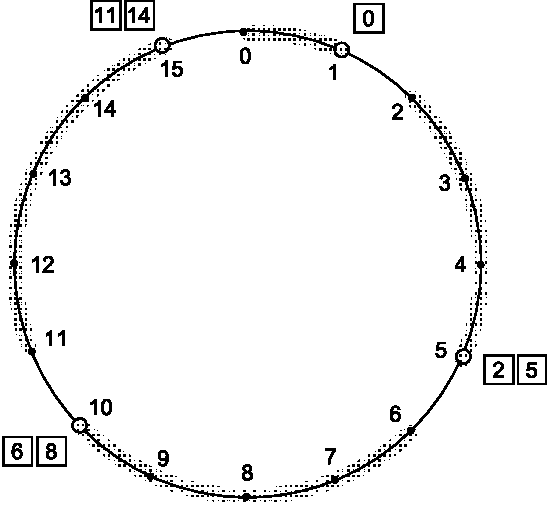
\includegraphics[width=0.4\textwidth]{pictures/pic0}\\
%  \caption[Example of a $4$-bit Chord identifier circle]{Example of a $4$-bit Chord identifier circle.
%  The responsibility ranges for each peer are accentuated in light gray}\label{fig:pic0}
%\end{figure}
%Es lassen sich auch mehrere Bilder nebeneinander platzieren wie z.B. in Abbildung
%\ref{fig:multipic} zu sehen ist.
%\begin{figure}[hpbt]
% \centering
%  %%----start of first subfigure----
%  \subfloat[FIFO size limited to 20 entries]{
%   \label{fig:multipic:a} %% label for first subfigure
%   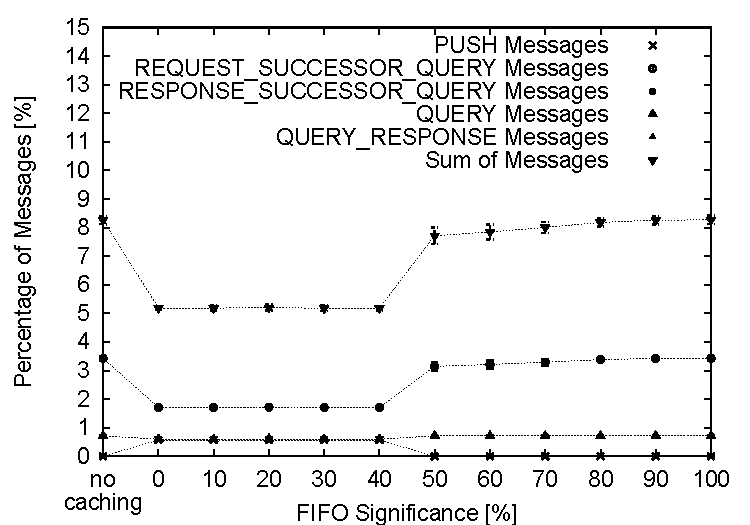
\includegraphics[width=0.48\linewidth]{pic1}}
%  \hspace{0.01\textwidth}
%  %%----start of second subfigure----
%  \subfloat[FIFO size limited to 30 entries]{
%   \label{fig:multipic:b} %% label for second subfigure
%   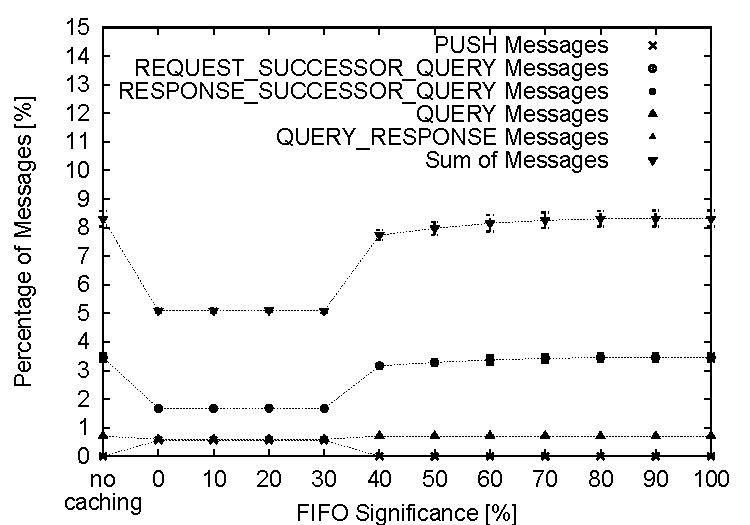
\includegraphics[width=0.48\linewidth]{pic2}}\\[0pt] % horizontal break
%  %%----start of third subfigure----
%  \subfloat[FIFO size limited to 40 entries]{
%   \label{fig:multipic:c} %% label for third subfigure
%   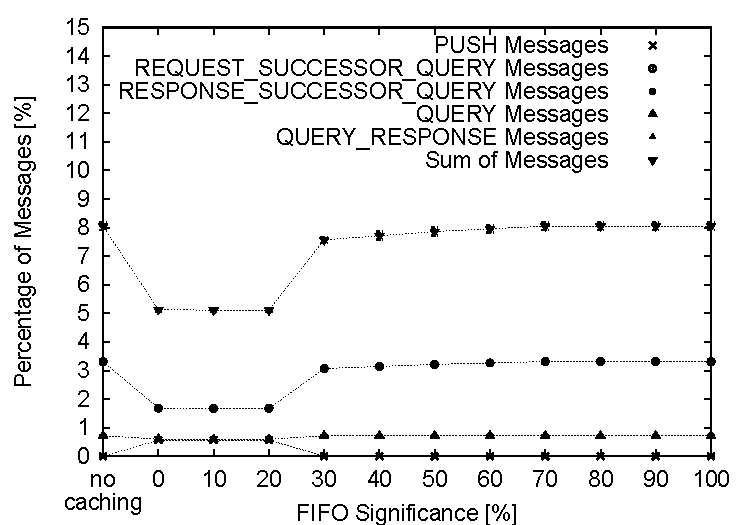
\includegraphics[width=0.48\linewidth]{pic3}}
%  \hspace{0.01\textwidth}
%  %%----start of fourth subfigure----
%  \subfloat[FIFO size limited to 50 entries]{
%   \label{fig:multipic:d} %% label for fourth subfigure
%   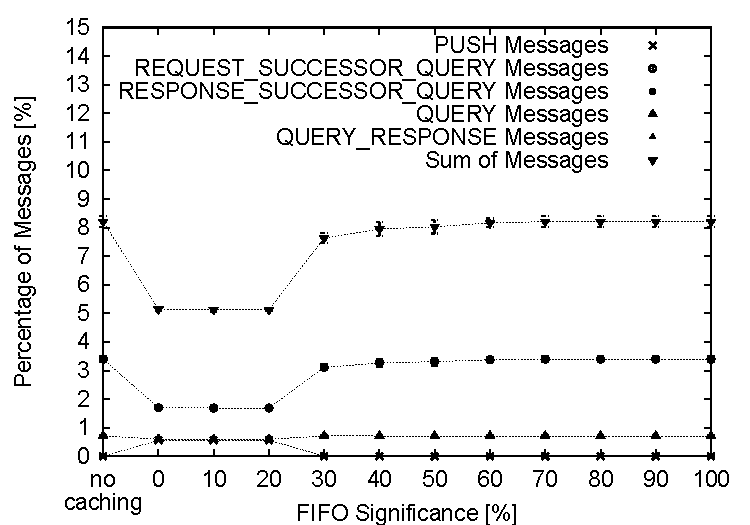
\includegraphics[width=0.48\linewidth]{pic4}}
% \caption[Observed message fractions and 95\% confidence intervals for Chord]{Observed message fractions and 95\% confidence intervals for Chord without the influence of churn. The FIFO capacity varies from 20 (\ref{fig:multipic:a}) -- 50 (\ref{fig:multipic:d}) entries (decadic steps).}
% \label{fig:multipic} %% label for entire figure
%\end{figure}
%
%\subsection{Programm Code}
%Eine elegante Möglichkeit, Programmtext einzubinden, lässt sich mit dem listings-Paket erreichen.
%Das \verb|HelloWorld| Programm aus Listing \ref{lst:hw} hat in Zeile \ref{line:hw3} übrigens einen Programmierfehler.
%\begin{lstlisting}[float=htp,caption=Hello World,label=lst:hw,language=Java, numbers=left, numberstyle=\tiny, stepnumber=2, numbersep=8pt, escapeinside={//@}{@//},backgroundcolor=\color{yellow},xleftmargin=3ex,xrightmargin=1ex]
%public class HelloWorld {
%    public static void main(String[] args) {
%        Syste.out.println("Hello, World"); //@\label{line:hw3}@//
%    }
%}
%\end{lstlisting}